\section{intro}

The last type of PF particle candidates to be reconstructed are hadrons. which are composite particles made up of quarks and gluons are stopped by the HCAL.
Some hadrons start showering in ECAL, and as mentioned in previous chapter that ECAL is well calibrated for EM particles, but not for hadrons.  (explain why, describe hadronic showers briefly + expand more on the reasons behind HCAL calibration). To accurately reconstruct these candidates, a correction for HCAL cluster energy needs to be applied after ECAL cluster calibration. 

This chapter similarly to the previous one presents the used ML method and datasets in performing the PF HCAL cluster energy regression.

\section{datasets description}

we privately generate single Pions samples: with E range 2-200 GeV,200-500 GeV and under 126X conditions.

we categorize particles depending on where the pion will start showering: H-hadrons where are particles that do not start a nuclear interaction in ECAL (hadronic shower) and EH-hadrons are particles that start showering in ECAL. the eta and phi of the Pions are the position at the ECAL entrance propagating through the tracker. (Maybe add more details related hadronic showers)

\section{PF cluster regression  using GNN}

Hadronic showers in the CMS detector have both electromagnetic and hadronic components. These showers are not fully contained in the ECAL but extend to HCAL. The reconstructed energy of hadrons is the sum of all reconstructed hits (offline, PF reconstruct the RAW data) from the ECAL and HCAL. 

Cluster Energy is reconstructed using both classical method (chi square) and DRN (based on GNN). 
Then for a given bin of true energy we fit the distribution of total RAW energy with Gaussian then we obtain: mu (mean energy) and std deviation.

Finally, we calculate: Resolution: (std/mu) which represent a measure of accuracy HCAL 
and Response of HCAL:  [(mu/E true) -1] : which is measurement of precision of HCAL 
(we can see that is not linear, another reason why the calibration of HCAL is not easy).

\section{results}
we present the results of response and resolution (from DRN vs Chi2) in  both Barrel region and endcap region.

\subsection{EH Hadrons}
the presented results are for the training target ratioflip
\begin{figure}
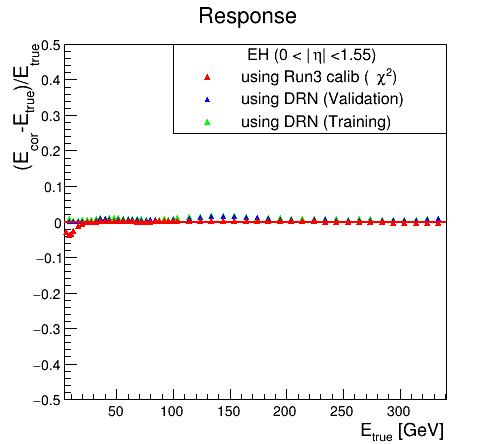
\includegraphics[width=0.495\textwidth]{./plots_pdf/HCAL_plots/Trained_target_ratioflip_0_500_10/pdf/EH_barrel/barrel_corrEtaBarrelEcalHcal.png}
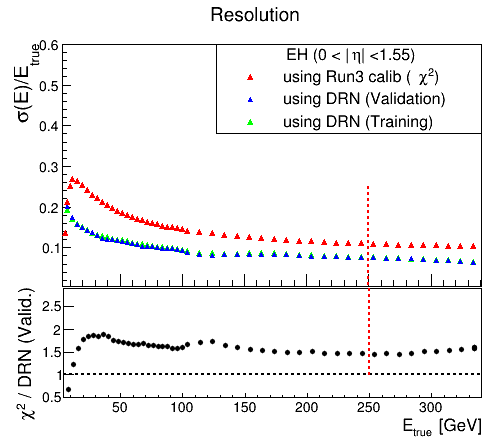
\includegraphics[width=0.495\textwidth]{./plots_pdf/HCAL_plots/Trained_target_ratioflip_0_500_10/pdf/EH_barrel/barrel_corrEtaBarrelEcalHcal_reso.png}
\caption{EH - barrel - target ratioflip}                                                                                                                                               
\end{figure}                                                                                                                                                                      

\begin{figure}                                                                                                                                                                   
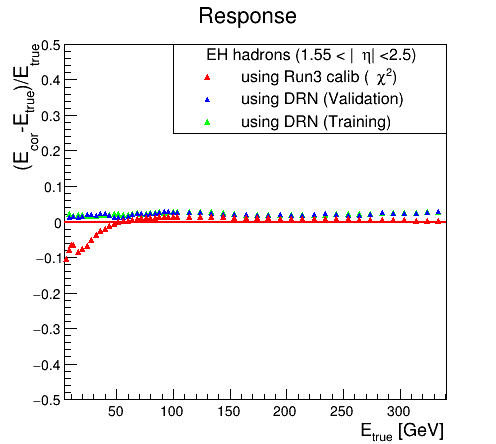
\includegraphics[width=0.495\textwidth]{./plots_pdf/HCAL_plots/Trained_target_ratioflip_0_500_10/pdf/EH_ec_in/EC_within_tracker_corrEtaEndcapEcalHcal.png}
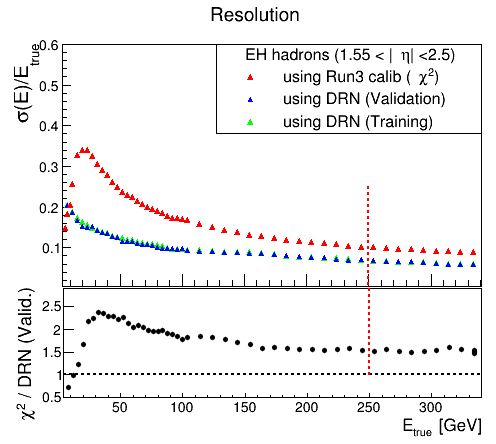
\includegraphics[width=0.495\textwidth]{./plots_pdf/HCAL_plots/Trained_target_ratioflip_0_500_10/pdf/EH_ec_in/EC_within_tracker_corrEtaEndcapEcalHcal_reso.png}
\caption{EH - endcap within tracker - target ratioflip}
\end{figure}


\begin{figure}
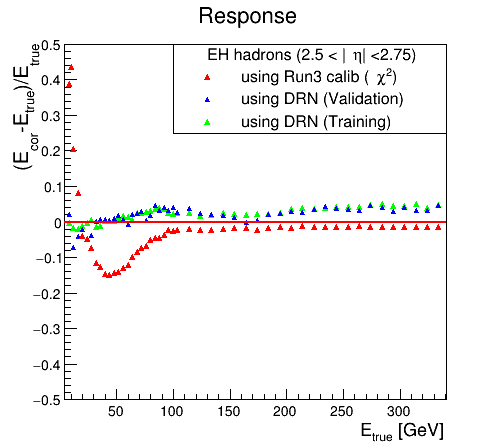
\includegraphics[width=0.495\textwidth]{./plots_pdf/HCAL_plots/Trained_target_ratioflip_0_500_10/pdf/EH_ec_out/EC_outside_tracker_corrEtaEndcapEcalHcal.png}
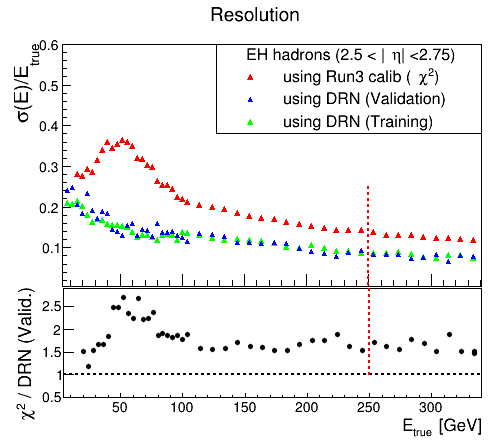
\includegraphics[width=0.495\textwidth]{./plots_pdf/HCAL_plots/Trained_target_ratioflip_0_500_10/pdf/EH_ec_out/EC_outside_tracker_corrEtaEndcapEcalHcal_reso.png}
\caption{EH - endcap outside the tracker - target ratioflip}
\end{figure}

\begin{figure}
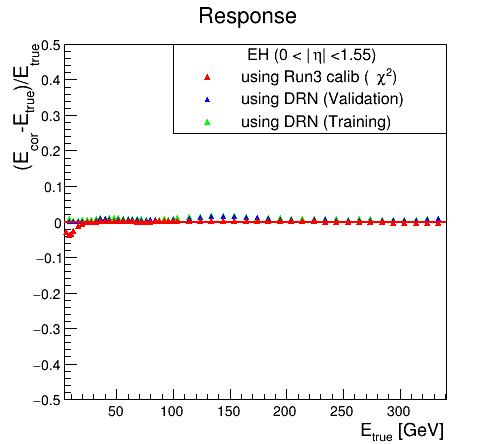
\includegraphics[width=0.495\textwidth]{./plots_pdf/HCAL_plots/Trained_target_ratioflip_0_500_10/pdf/EH_barrel/barrel_corrEtaBarrelEcalHcal.png}
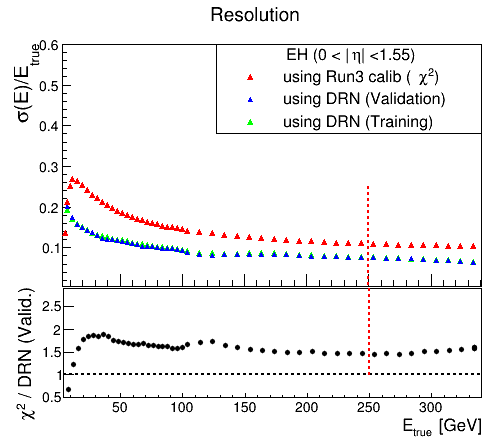
\includegraphics[width=0.495\textwidth]{./plots_pdf/HCAL_plots/Trained_target_ratioflip_0_500_10/pdf/EH_barrel/barrel_corrEtaBarrelEcalHcal_reso.png}
\caption{EH - barrel - target logratioflip}
\end{figure}

\begin{figure}
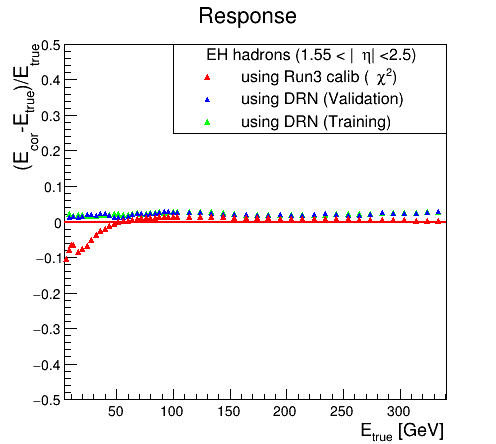
\includegraphics[width=0.495\textwidth]{./plots_pdf/HCAL_plots/Trained_target_ratioflip_0_500_10/pdf/EH_ec_in/EC_within_tracker_corrEtaEndcapEcalHcal.png}
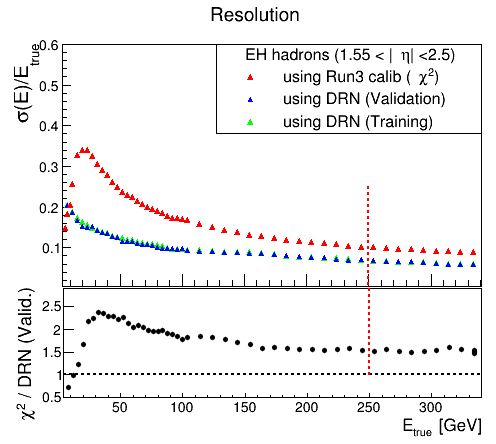
\includegraphics[width=0.495\textwidth]{./plots_pdf/HCAL_plots/Trained_target_ratioflip_0_500_10/pdf/EH_ec_in/EC_within_tracker_corrEtaEndcapEcalHcal_reso.png}
\caption{EH - endcap within tracker - target logratioflip}
\end{figure}


\begin{figure}
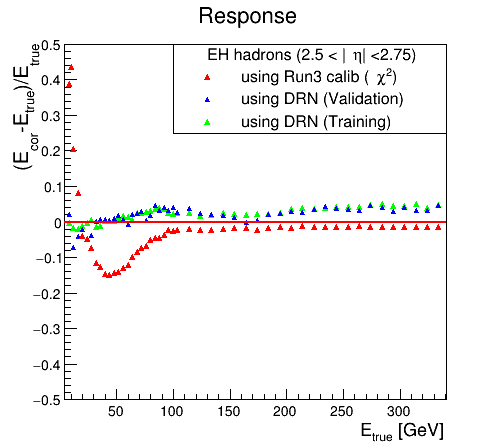
\includegraphics[width=0.495\textwidth]{./plots_pdf/HCAL_plots/Trained_target_ratioflip_0_500_10/pdf/EH_ec_out/EC_outside_tracker_corrEtaEndcapEcalHcal.png}
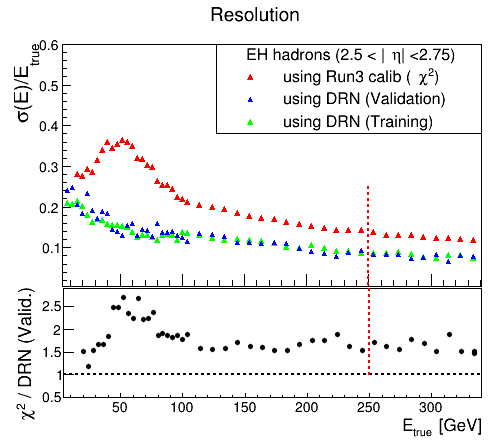
\includegraphics[width=0.495\textwidth]{./plots_pdf/HCAL_plots/Trained_target_ratioflip_0_500_10/pdf/EH_ec_out/EC_outside_tracker_corrEtaEndcapEcalHcal_reso.png}
\caption{EH - endcap outside the tracker - target logratioflip}
\end{figure}

\begin{figure}
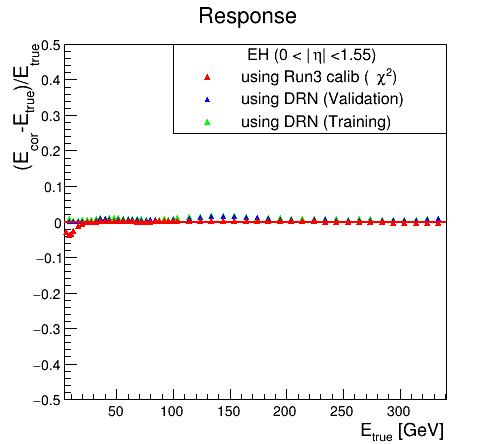
\includegraphics[width=0.495\textwidth]{./plots_pdf/HCAL_plots/Trained_target_ratioflip_0_500_10/pdf/EH_barrel/barrel_corrEtaBarrelEcalHcal.png}
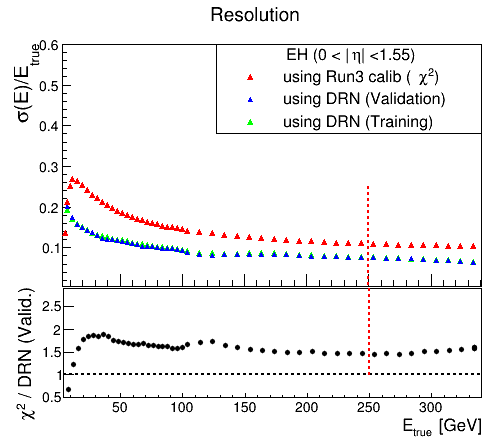
\includegraphics[width=0.495\textwidth]{./plots_pdf/HCAL_plots/Trained_target_ratioflip_0_500_10/pdf/EH_barrel/barrel_corrEtaBarrelEcalHcal_reso.png}
\caption{EH - barrel - target_ratio}                                                                                                                                               
\end{figure}                                                                                                                                                                      

\begin{figure}                                                                                                                                                                   
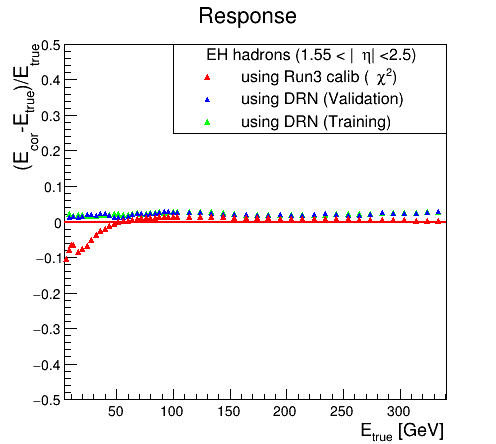
\includegraphics[width=0.495\textwidth]{./plots_pdf/HCAL_plots/Trained_target_ratioflip_0_500_10/pdf/EH_ec_in/EC_within_tracker_corrEtaEndcapEcalHcal.png}
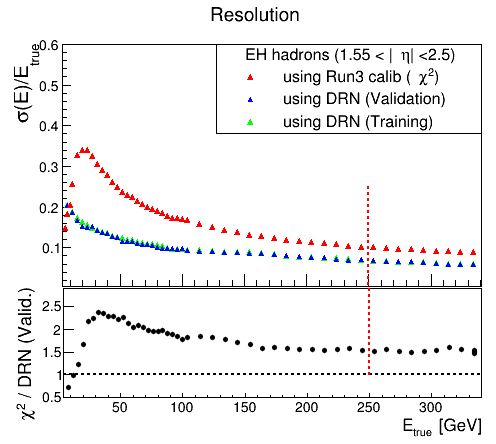
\includegraphics[width=0.495\textwidth]{./plots_pdf/HCAL_plots/Trained_target_ratioflip_0_500_10/pdf/EH_ec_in/EC_within_tracker_corrEtaEndcapEcalHcal_reso.png}
\caption{EH - endcap within tracker - target_ratio}
\end{figure}


\begin{figure}
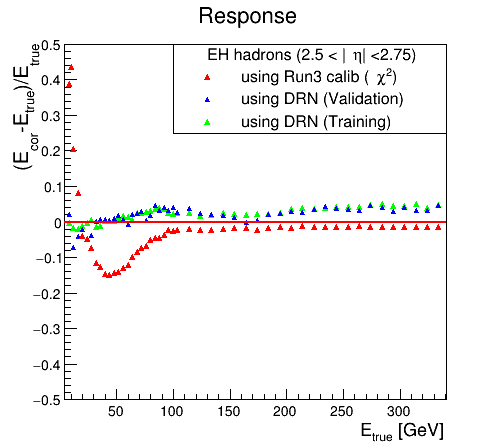
\includegraphics[width=0.495\textwidth]{./plots_pdf/HCAL_plots/Trained_target_ratioflip_0_500_10/pdf/EH_ec_out/EC_outside_tracker_corrEtaEndcapEcalHcal.png}
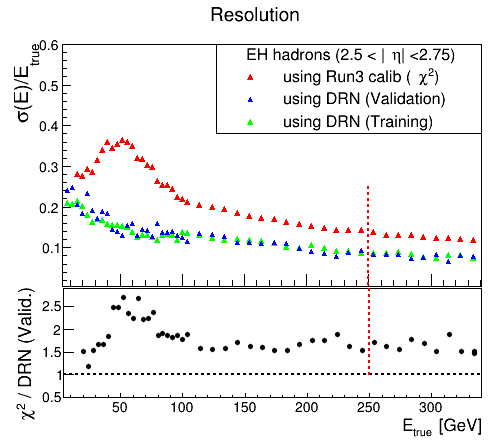
\includegraphics[width=0.495\textwidth]{./plots_pdf/HCAL_plots/Trained_target_ratioflip_0_500_10/pdf/EH_ec_out/EC_outside_tracker_corrEtaEndcapEcalHcal_reso.png}
\caption{EH - endcap outside the tracker - target_ratio}
\end{figure}

\begin{figure}
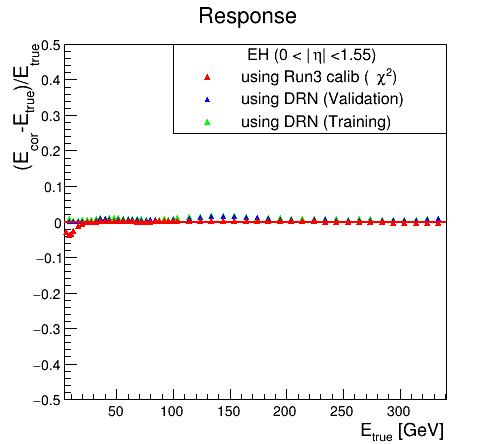
\includegraphics[width=0.495\textwidth]{./plots_pdf/HCAL_plots/Trained_target_ratioflip_0_500_10/pdf/EH_barrel/barrel_corrEtaBarrelEcalHcal.png}
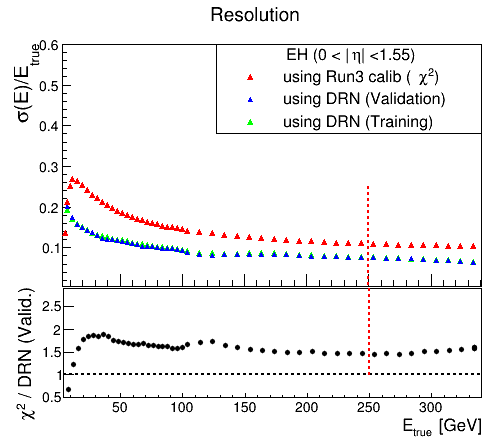
\includegraphics[width=0.495\textwidth]{./plots_pdf/HCAL_plots/Trained_target_ratioflip_0_500_10/pdf/EH_barrel/barrel_corrEtaBarrelEcalHcal_reso.png}
%\caption{EH - barrel - target trueE}
%\end{figure}

%\begin{figure}
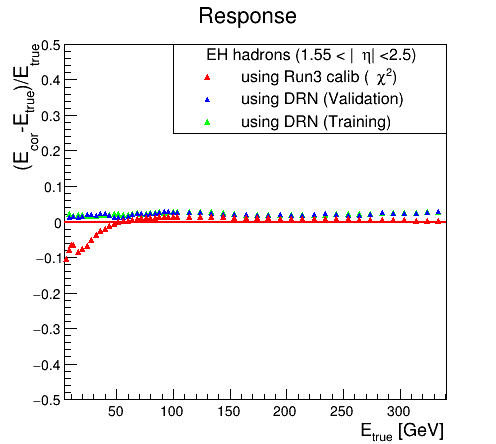
\includegraphics[width=0.495\textwidth]{./plots_pdf/HCAL_plots/Trained_target_ratioflip_0_500_10/pdf/EH_ec_in/EC_within_tracker_corrEtaEndcapEcalHcal.png}
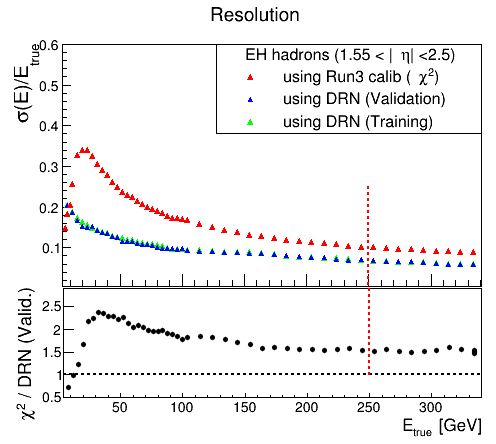
\includegraphics[width=0.495\textwidth]{./plots_pdf/HCAL_plots/Trained_target_ratioflip_0_500_10/pdf/EH_ec_in/EC_within_tracker_corrEtaEndcapEcalHcal_reso.png}
%\caption{EH - endcap within tracker - target trueE}
%\end{figure}


%\begin{figure}
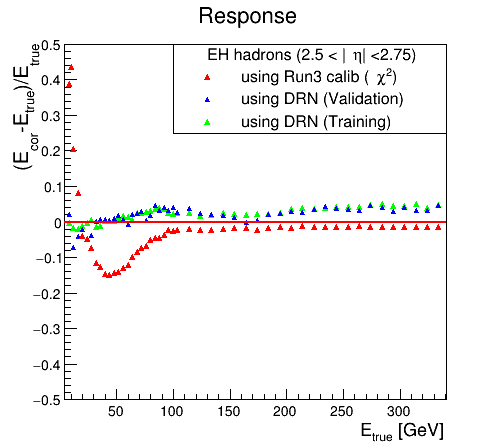
\includegraphics[width=0.495\textwidth]{./plots_pdf/HCAL_plots/Trained_target_ratioflip_0_500_10/pdf/EH_ec_out/EC_outside_tracker_corrEtaEndcapEcalHcal.png}
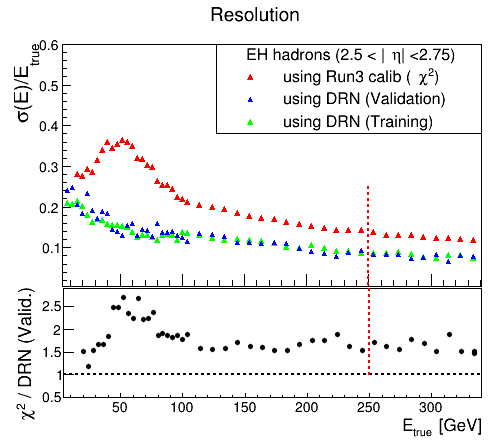
\includegraphics[width=0.495\textwidth]{./plots_pdf/HCAL_plots/Trained_target_ratioflip_0_500_10/pdf/EH_ec_out/EC_outside_tracker_corrEtaEndcapEcalHcal_reso.png}
\caption{EH - (top) barrel, (middle) endcap within tracker, (bottom) endcap outside the tracker - target trueE}
\label{fig:EH_trueE}
\end{figure}


\subsection{H hadrons}
\begin{figure}
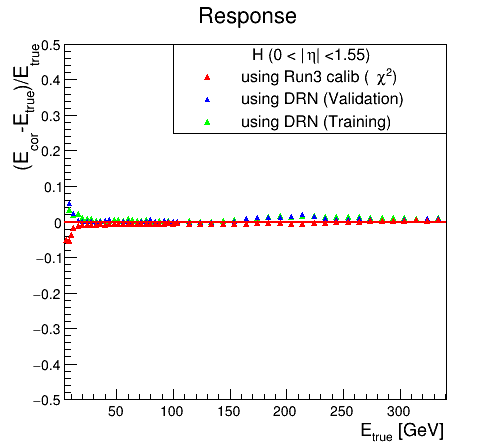
\includegraphics[width=0.495\textwidth]{./plots_pdf/HCAL_plots/Trained_target_ratioflip_0_500_10/pdf/H_barrel/barrel_corrEtaBarrelHcal.png}
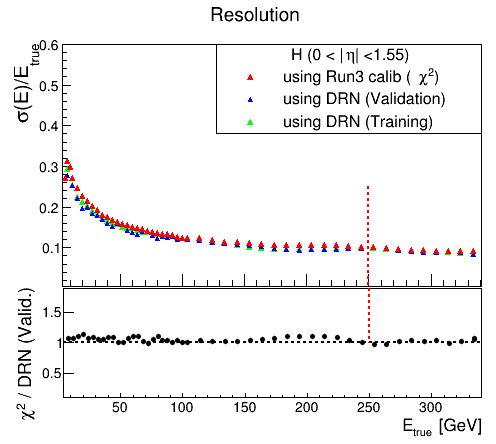
\includegraphics[width=0.495\textwidth]{./plots_pdf/HCAL_plots/Trained_target_ratioflip_0_500_10/pdf/H_barrel/barrel_corrEtaBarrelHcal_reso.png}

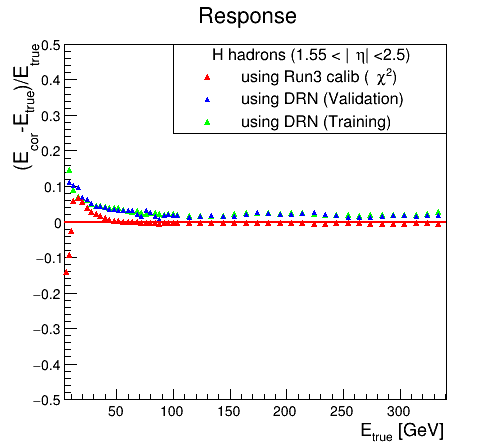
\includegraphics[width=0.495\textwidth]{./plots_pdf/HCAL_plots/Trained_target_ratioflip_0_500_10/pdf/H_ec_in/EC_within_tracker_corrEtaEndcapHcal.png}
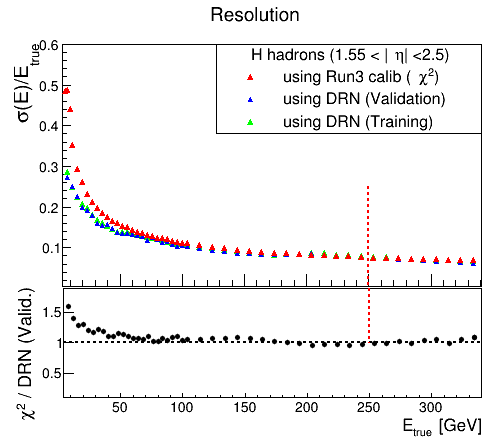
\includegraphics[width=0.495\textwidth]{./plots_pdf/HCAL_plots/Trained_target_ratioflip_0_500_10/pdf/H_ec_in/EC_within_tracker_corrEtaEndcapHcal_reso.png}

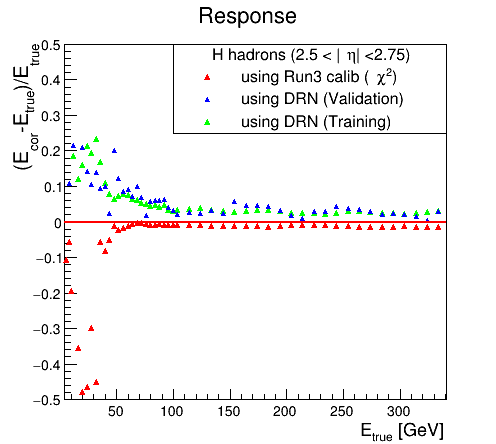
\includegraphics[width=0.495\textwidth]{./plots_pdf/HCAL_plots/Trained_target_ratioflip_0_500_10/pdf/H_ec_out/EC_outside_tracker_corrEtaEndcapHcal.png}
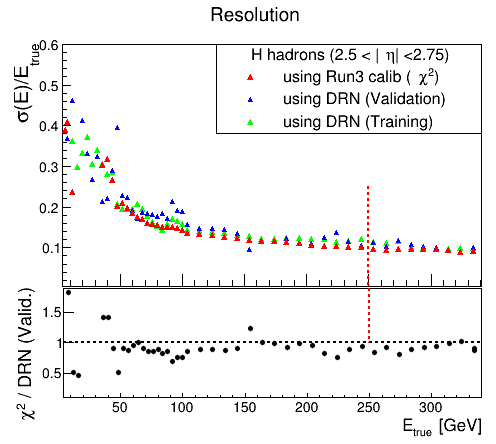
\includegraphics[width=0.495\textwidth]{./plots_pdf/HCAL_plots/Trained_target_ratioflip_0_500_10/pdf/H_ec_out/EC_outside_tracker_corrEtaEndcapHcal_reso.png}

\caption[Energy response (resolution) of the PF H-hadron cluster training traget ratioflip]{H - (top) barrel , (middle) endcap within tracker, (bottom) endcap outside the tracker - target ratioflip}
\label{fig:H_ratioflip}
\end{figure}

\begin{figure}
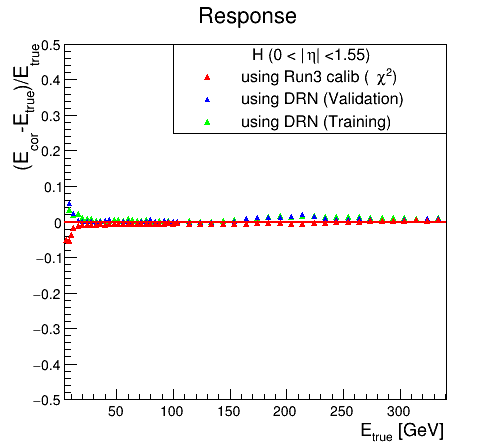
\includegraphics[width=0.495\textwidth]{./plots_pdf/HCAL_plots/Trained_target_ratioflip_0_500_10/pdf/H_barrel/barrel_corrEtaBarrelHcal.png}
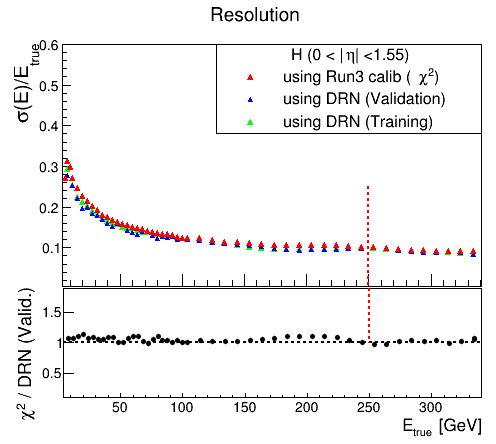
\includegraphics[width=0.495\textwidth]{./plots_pdf/HCAL_plots/Trained_target_ratioflip_0_500_10/pdf/H_barrel/barrel_corrEtaBarrelHcal_reso.png}
\caption{H - barrel - target_logratioflip}                                                                                                                                               
\end{figure}


\begin{figure}                                                                                                                                                               
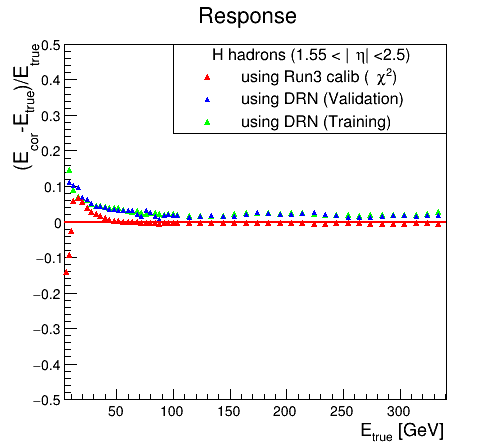
\includegraphics[width=0.495\textwidth]{./plots_pdf/HCAL_plots/Trained_target_ratioflip_0_500_10/pdf/H_ec_in/EC_within_tracker_corrEtaEndcapHcal.png}
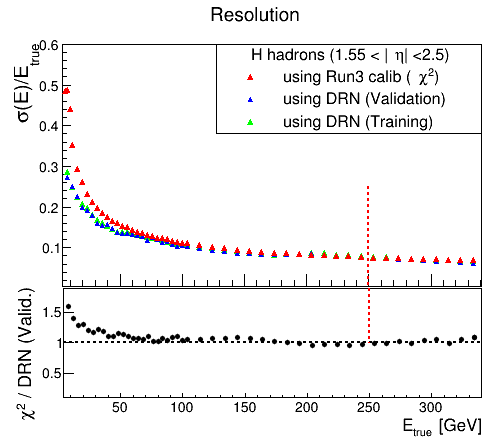
\includegraphics[width=0.495\textwidth]{./plots_pdf/HCAL_plots/Trained_target_ratioflip_0_500_10/pdf/H_ec_in/EC_within_tracker_corrEtaEndcapHcal_reso.png}
\caption{H - endcap within tracker - target_logratioflip}
\end{figure}


\begin{figure}
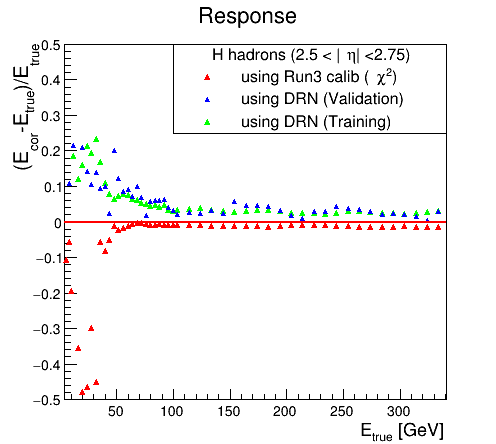
\includegraphics[width=0.495\textwidth]{./plots_pdf/HCAL_plots/Trained_target_ratioflip_0_500_10/pdf/H_ec_out/EC_outside_tracker_corrEtaEndcapHcal.png}
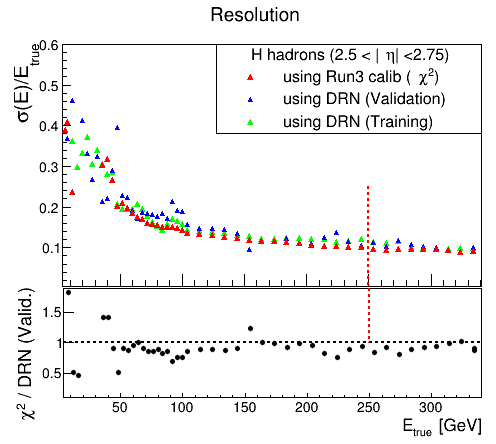
\includegraphics[width=0.495\textwidth]{./plots_pdf/HCAL_plots/Trained_target_ratioflip_0_500_10/pdf/H_ec_out/EC_outside_tracker_corrEtaEndcapHcal_reso.png}
\caption{H - endcap outside the tracker - target_logratioflip}
\end{figure}

\begin{figure}
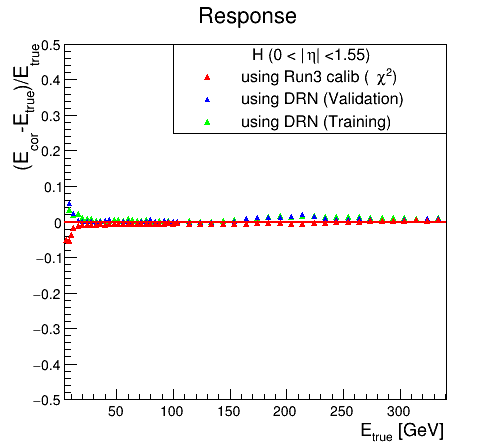
\includegraphics[width=0.495\textwidth]{./plots_pdf/HCAL_plots/Trained_target_ratioflip_0_500_10/pdf/H_barrel/barrel_corrEtaBarrelHcal.png}
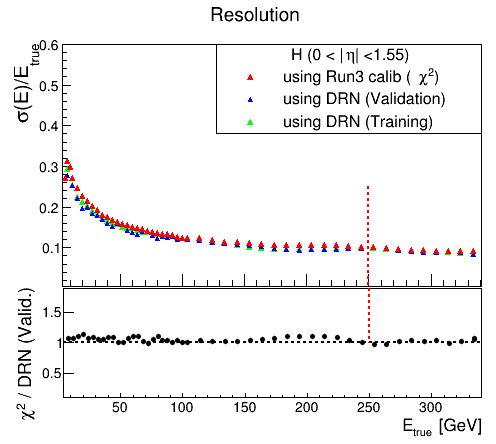
\includegraphics[width=0.495\textwidth]{./plots_pdf/HCAL_plots/Trained_target_ratioflip_0_500_10/pdf/H_barrel/barrel_corrEtaBarrelHcal_reso.png}
%\caption{H - barrel - target ratio}
%\end{figure}


%\begin{figure}
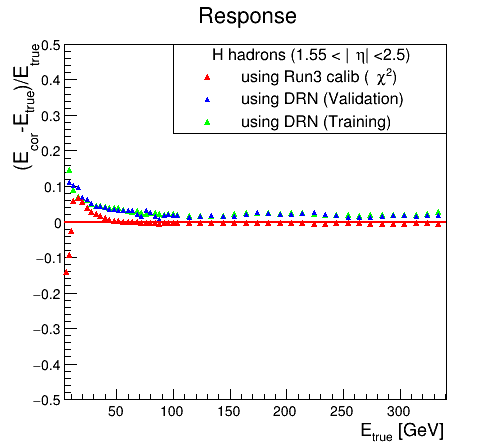
\includegraphics[width=0.495\textwidth]{./plots_pdf/HCAL_plots/Trained_target_ratioflip_0_500_10/pdf/H_ec_in/EC_within_tracker_corrEtaEndcapHcal.png}
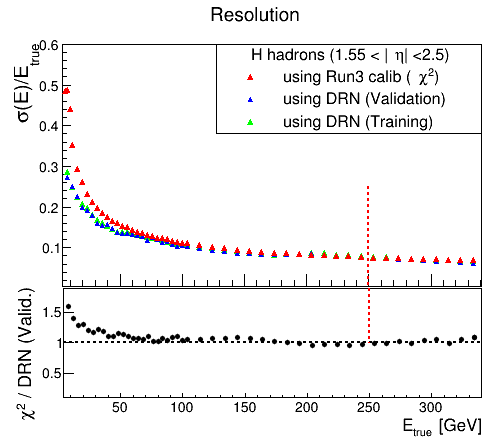
\includegraphics[width=0.495\textwidth]{./plots_pdf/HCAL_plots/Trained_target_ratioflip_0_500_10/pdf/H_ec_in/EC_within_tracker_corrEtaEndcapHcal_reso.png}
%\caption{H - endcap within tracker - target ratio}
%\end{figure}


%\begin{figure}
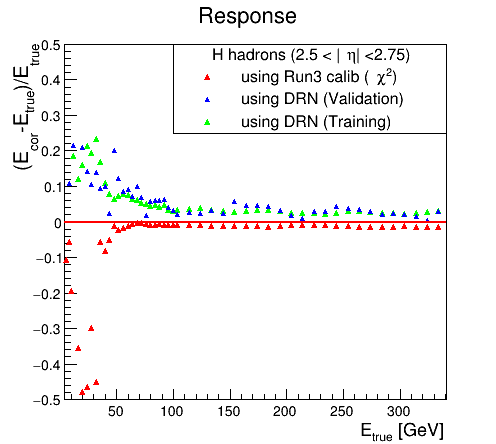
\includegraphics[width=0.495\textwidth]{./plots_pdf/HCAL_plots/Trained_target_ratioflip_0_500_10/pdf/H_ec_out/EC_outside_tracker_corrEtaEndcapHcal.png}
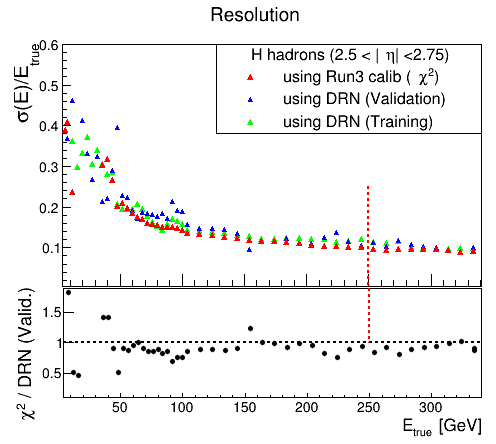
\includegraphics[width=0.495\textwidth]{./plots_pdf/HCAL_plots/Trained_target_ratioflip_0_500_10/pdf/H_ec_out/EC_outside_tracker_corrEtaEndcapHcal_reso.png}
\caption{H - (top) barrel, (middle) endcap within tracker, (bottom) endcap outside the tracker - target ratio}
\end{figure}

\begin{figure}
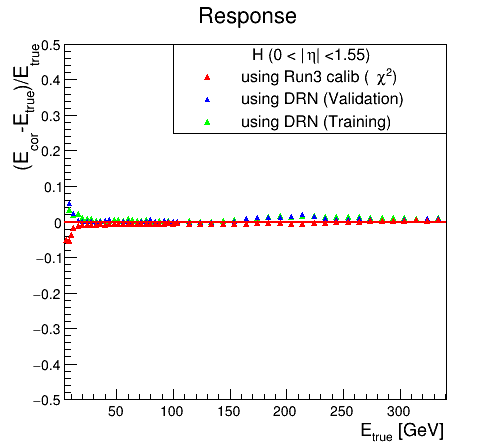
\includegraphics[width=0.495\textwidth]{./plots_pdf/HCAL_plots/Trained_target_ratioflip_0_500_10/pdf/H_barrel/barrel_corrEtaBarrelHcal.png}
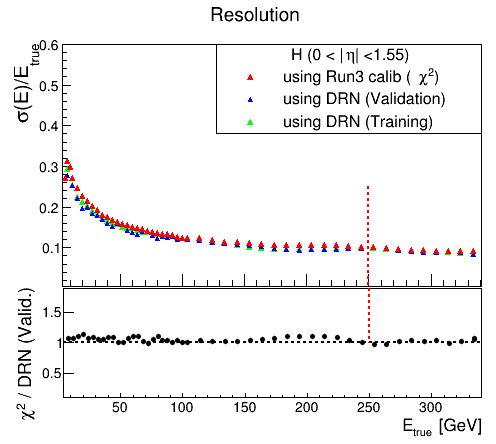
\includegraphics[width=0.495\textwidth]{./plots_pdf/HCAL_plots/Trained_target_ratioflip_0_500_10/pdf/H_barrel/barrel_corrEtaBarrelHcal_reso.png}
\caption{H - barrel - target_trueE}                                                                                                                                               
\end{figure}


\begin{figure}                                                                                                                                                               
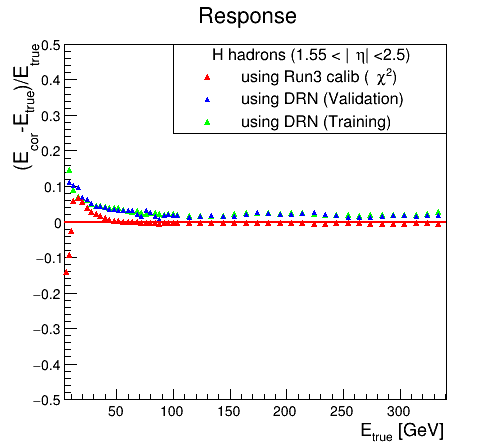
\includegraphics[width=0.495\textwidth]{./plots_pdf/HCAL_plots/Trained_target_ratioflip_0_500_10/pdf/H_ec_in/EC_within_tracker_corrEtaEndcapHcal.png}
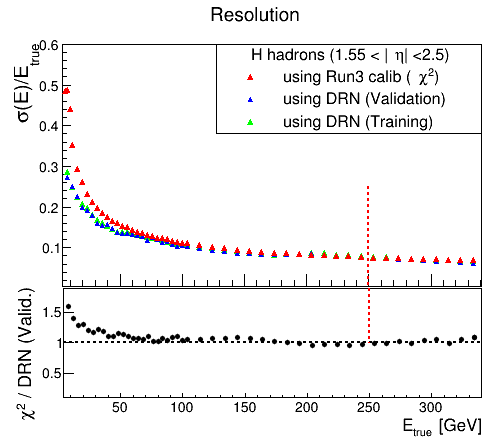
\includegraphics[width=0.495\textwidth]{./plots_pdf/HCAL_plots/Trained_target_ratioflip_0_500_10/pdf/H_ec_in/EC_within_tracker_corrEtaEndcapHcal_reso.png}
\caption{H - endcap within tracker - target_trueE}
\end{figure}


\begin{figure}
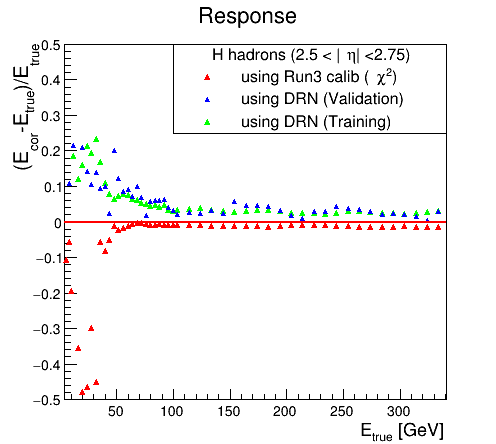
\includegraphics[width=0.495\textwidth]{./plots_pdf/HCAL_plots/Trained_target_ratioflip_0_500_10/pdf/H_ec_out/EC_outside_tracker_corrEtaEndcapHcal.png}
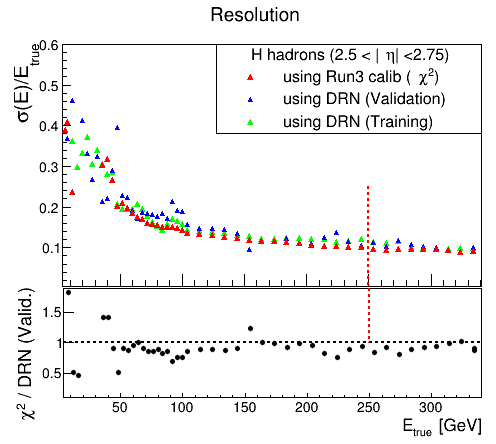
\includegraphics[width=0.495\textwidth]{./plots_pdf/HCAL_plots/Trained_target_ratioflip_0_500_10/pdf/H_ec_out/EC_outside_tracker_corrEtaEndcapHcal_reso.png}
\caption{H - endcap outside the tracker - target_trueE}
\end{figure}

